
%%%%%%%%%%%%%%%%%% PREAMBULE %%%%%%%%%%%%%%%%%%

\documentclass[aspectratio=169,utf8]{beamer}
%\documentclass[aspectratio=169,handout]{beamer}

\usetheme{Boadilla}
%\usecolortheme{seahorse}
\usecolortheme[RGB={245,66,24}]{structure}
\useoutertheme{infolines}

% packages
\usepackage{amsfonts,amsmath,amssymb,amsthm}
\usepackage[utf8]{inputenc}
\usepackage[T1]{fontenc}
\usepackage{lmodern}

\usepackage[francais]{babel}
\usepackage{fancybox}
\usepackage{graphicx}

\usepackage{float}
\usepackage{xfrac}

%\usepackage[usenames, x11names]{xcolor}
\usepackage{tikz}
\usepackage{pgfplots}
\usepackage{datetime}



%-----  Package unités -----
\usepackage{siunitx}
\sisetup{locale = FR,detect-all,per-mode = symbol}

%\usepackage{mathptmx}
%\usepackage{fouriernc}
%\usepackage{newcent}
%\usepackage[mathcal,mathbf]{euler}

%\usepackage{palatino}
%\usepackage{newcent}
% \usepackage[mathcal,mathbf]{euler}



% \usepackage{hyperref}
% \hypersetup{colorlinks=true, linkcolor=blue, urlcolor=blue,
% pdftitle={Exo7 - Exercices de mathématiques}, pdfauthor={Exo7}}


%section
% \usepackage{sectsty}
% \allsectionsfont{\bf}
%\sectionfont{\color{Tomato3}\upshape\selectfont}
%\subsectionfont{\color{Tomato4}\upshape\selectfont}

%----- Ensembles : entiers, reels, complexes -----
\newcommand{\Nn}{\mathbb{N}} \newcommand{\N}{\mathbb{N}}
\newcommand{\Zz}{\mathbb{Z}} \newcommand{\Z}{\mathbb{Z}}
\newcommand{\Qq}{\mathbb{Q}} \newcommand{\Q}{\mathbb{Q}}
\newcommand{\Rr}{\mathbb{R}} \newcommand{\R}{\mathbb{R}}
\newcommand{\Cc}{\mathbb{C}} 
\newcommand{\Kk}{\mathbb{K}} \newcommand{\K}{\mathbb{K}}

%----- Modifications de symboles -----
\renewcommand{\epsilon}{\varepsilon}
\renewcommand{\Re}{\mathop{\text{Re}}\nolimits}
\renewcommand{\Im}{\mathop{\text{Im}}\nolimits}
%\newcommand{\llbracket}{\left[\kern-0.15em\left[}
%\newcommand{\rrbracket}{\right]\kern-0.15em\right]}

\renewcommand{\ge}{\geqslant}
\renewcommand{\geq}{\geqslant}
\renewcommand{\le}{\leqslant}
\renewcommand{\leq}{\leqslant}
\renewcommand{\epsilon}{\varepsilon}

%----- Fonctions usuelles -----
\newcommand{\ch}{\mathop{\text{ch}}\nolimits}
\newcommand{\sh}{\mathop{\text{sh}}\nolimits}
\renewcommand{\tanh}{\mathop{\text{th}}\nolimits}
\newcommand{\cotan}{\mathop{\text{cotan}}\nolimits}
\newcommand{\Arcsin}{\mathop{\text{arcsin}}\nolimits}
\newcommand{\Arccos}{\mathop{\text{arccos}}\nolimits}
\newcommand{\Arctan}{\mathop{\text{arctan}}\nolimits}
\newcommand{\Argsh}{\mathop{\text{argsh}}\nolimits}
\newcommand{\Argch}{\mathop{\text{argch}}\nolimits}
\newcommand{\Argth}{\mathop{\text{argth}}\nolimits}
\newcommand{\pgcd}{\mathop{\text{pgcd}}\nolimits} 


%----- Commandes divers ------
\newcommand{\ii}{\mathrm{i}}
\newcommand{\dd}{\text{d}}
\newcommand{\id}{\mathop{\text{id}}\nolimits}
\newcommand{\Ker}{\mathop{\text{Ker}}\nolimits}
\newcommand{\Card}{\mathop{\text{Card}}\nolimits}
\newcommand{\Vect}{\mathop{\text{Vect}}\nolimits}
\newcommand{\Mat}{\mathop{\text{Mat}}\nolimits}
\newcommand{\rg}{\mathop{\text{rg}}\nolimits}
\newcommand{\tr}{\mathop{\text{tr}}\nolimits}


%----- Structure des exercices ------

\newtheoremstyle{styleexo}% name
{2ex}% Space above
{3ex}% Space below
{}% Body font
{}% Indent amount 1
{\bfseries} % Theorem head font
{}% Punctuation after theorem head
{\newline}% Space after theorem head 2
{}% Theorem head spec (can be left empty, meaning ‘normal’)

%\theoremstyle{styleexo}
\newtheorem{exo}{Exercice}
\newtheorem{ind}{Indications}
\newtheorem{cor}{Correction}


\newcommand{\exercice}[1]{} \newcommand{\finexercice}{}
%\newcommand{\exercice}[1]{{\tiny\texttt{#1}}\vspace{-2ex}} % pour afficher le numero absolu, l'auteur...
\newcommand{\enonce}{\begin{exo}} \newcommand{\finenonce}{\end{exo}}
\newcommand{\indication}{\begin{ind}} \newcommand{\finindication}{\end{ind}}
\newcommand{\correction}{\begin{cor}} \newcommand{\fincorrection}{\end{cor}}

\newcommand{\noindication}{\stepcounter{ind}}
\newcommand{\nocorrection}{\stepcounter{cor}}

\newcommand{\fiche}[1]{} \newcommand{\finfiche}{}
\newcommand{\titre}[1]{\centerline{\large \bf #1}}
\newcommand{\addcommand}[1]{}
\newcommand{\video}[1]{}

% Marge
\newcommand{\mymargin}[1]{\marginpar{{\small #1}}}

\def\noqed{\renewcommand{\qedsymbol}{}}


%----- Presentation ------
\setlength{\parindent}{0cm}

%\newcommand{\ExoSept}{\href{http://exo7.emath.fr}{\textbf{\textsf{Exo7}}}}

\definecolor{myred}{rgb}{0.93,0.26,0}
\definecolor{myorange}{rgb}{0.97,0.58,0}
\definecolor{myyellow}{rgb}{1,0.86,0}

\newcommand{\LogoExoSept}[1]{  % input : echelle
{\usefont{U}{cmss}{bx}{n}
\begin{tikzpicture}[scale=0.1*#1,transform shape]
  \fill[color=myorange] (0,0)--(4,0)--(4,-4)--(0,-4)--cycle;
  \fill[color=myred] (0,0)--(0,3)--(-3,3)--(-3,0)--cycle;
  \fill[color=myyellow] (4,0)--(7,4)--(3,7)--(0,3)--cycle;
  \node[scale=5] at (3.5,3.5) {Exo7};
\end{tikzpicture}}
}


\newcommand{\debutmontitre}{
  \author{} \date{} 
  \thispagestyle{empty}
  \hspace*{-10ex}
  \begin{minipage}{\textwidth}
    \titlepage  
  \vspace*{-2.5cm}
  \begin{center}
    \LogoExoSept{2.5}
  \end{center}
  \end{minipage}

  \vspace*{-0cm}
  
  % Astuce pour que le background ne soit pas discrétisé lors de la conversion pdf -> png
\begin{tikzpicture}
        \fill[opacity=0,green!60!black] (0,0)--++(0,0)--++(0,0)--++(0,0)--cycle; 
\end{tikzpicture}

% toc S'affiche trop tot :
% \tableofcontents[hideallsubsections, pausesections]
}

\newcommand{\finmontitre}{
  \end{frame}
  \setcounter{framenumber}{0}
} % ne marche pas pour une raison obscure

%----- Commandes supplementaires ------

% \usepackage[landscape]{geometry}
% \geometry{top=1cm, bottom=3cm, left=2cm, right=10cm, marginparsep=1cm
% }
% \usepackage[a4paper]{geometry}
% \geometry{top=2cm, bottom=2cm, left=2cm, right=2cm, marginparsep=1cm
% }

%\usepackage{standalone}


% New command Arnaud -- november 2011
\setbeamersize{text margin left=24ex}
% si vous modifier cette valeur il faut aussi
% modifier le decalage du titre pour compenser
% (ex : ici =+10ex, titre =-5ex

\theoremstyle{definition}
%\newtheorem{proposition}{Proposition}
%\newtheorem{exemple}{Exemple}
%\newtheorem{theoreme}{Théorème}
%\newtheorem{lemme}{Lemme}
%\newtheorem{corollaire}{Corollaire}
%\newtheorem*{remarque*}{Remarque}
%\newtheorem*{miniexercice}{Mini-exercices}
%\newtheorem{definition}{Définition}

% Commande tikz
\usetikzlibrary{calc}
\usetikzlibrary{patterns,arrows}
\usetikzlibrary{matrix}
\usetikzlibrary{fadings} 

%definition d'un terme
\newcommand{\defi}[1]{{\color{myorange}\textbf{\emph{#1}}}}
\newcommand{\evidence}[1]{{\color{blue}\textbf{\emph{#1}}}}
\newcommand{\assertion}[1]{\emph{\og#1\fg}}  % pour chapitre logique
%\renewcommand{\contentsname}{Sommaire}
\renewcommand{\contentsname}{}
\setcounter{tocdepth}{2}



%------ Figures ------

\def\myscale{1} % par défaut 
\newcommand{\myfigure}[2]{  % entrée : echelle, fichier figure
\def\myscale{#1}
\begin{center}
\footnotesize
{#2}
\end{center}}


%------ Encadrement ------

\usepackage{fancybox}


\newcommand{\mybox}[1]{
\setlength{\fboxsep}{7pt}
\begin{center}
\shadowbox{#1}
\end{center}}

\newcommand{\myboxinline}[1]{
\setlength{\fboxsep}{5pt}
\raisebox{-10pt}{
\shadowbox{#1}
}
}

%--------------- Commande beamer---------------
\newcommand{\beameronly}[1]{#1} % permet de mettre des pause dans beamer pas dans poly


\setbeamertemplate{navigation symbols}{}
\setbeamertemplate{footline}  % tiré du fichier beamerouterinfolines.sty
{
  \leavevmode%
  \hbox{%
  \begin{beamercolorbox}[wd=.333333\paperwidth,ht=2.25ex,dp=1ex,center]{author in head/foot}%
    % \usebeamerfont{author in head/foot}\insertshortauthor%~~(\insertshortinstitute)
    \usebeamerfont{section in head/foot}{\bf\insertshorttitle}
  \end{beamercolorbox}%
  \begin{beamercolorbox}[wd=.333333\paperwidth,ht=2.25ex,dp=1ex,center]{title in head/foot}%
    \usebeamerfont{section in head/foot}{\bf\insertsectionhead}
  \end{beamercolorbox}%
  \begin{beamercolorbox}[wd=.333333\paperwidth,ht=2.25ex,dp=1ex,right]{date in head/foot}%
    % \usebeamerfont{date in head/foot}\insertshortdate{}\hspace*{2em}
    \insertframenumber{} / \inserttotalframenumber\hspace*{2ex} 
  \end{beamercolorbox}}%
  \vskip0pt%
}


\definecolor{mygrey}{rgb}{0.5,0.5,0.5}
\setlength{\parindent}{0cm}
%\DeclareTextFontCommand{\helvetica}{\fontfamily{phv}\selectfont}

% background beamer
\definecolor{couleurhaut}{rgb}{0.85,0.9,1}  % creme
\definecolor{couleurmilieu}{rgb}{1,1,1}  % vert pale
\definecolor{couleurbas}{rgb}{0.85,0.9,1}  % blanc
\setbeamertemplate{background canvas}[vertical shading]%
[top=couleurhaut,middle=couleurmilieu,midpoint=0.4,bottom=couleurbas] 
%[top=fondtitre!05,bottom=fondtitre!60]



\makeatletter
\setbeamertemplate{theorem begin}
{%
  \begin{\inserttheoremblockenv}
  {%
    \inserttheoremheadfont
    \inserttheoremname
    \inserttheoremnumber
    \ifx\inserttheoremaddition\@empty\else\ (\inserttheoremaddition)\fi%
    \inserttheorempunctuation
  }%
}
\setbeamertemplate{theorem end}{\end{\inserttheoremblockenv}}

\newenvironment{theoreme}[1][]{%
   \setbeamercolor{block title}{fg=structure,bg=structure!40}
   \setbeamercolor{block body}{fg=black,bg=structure!10}
   \begin{block}{{\bf Th\'eor\`eme }#1}
}{%
   \end{block}%
}


\newenvironment{proposition}[1][]{%
   \setbeamercolor{block title}{fg=structure,bg=structure!40}
   \setbeamercolor{block body}{fg=black,bg=structure!10}
   \begin{block}{{\bf Proposition }#1}
}{%
   \end{block}%
}

\newenvironment{corollaire}[1][]{%
   \setbeamercolor{block title}{fg=structure,bg=structure!40}
   \setbeamercolor{block body}{fg=black,bg=structure!10}
   \begin{block}{{\bf Corollaire }#1}
}{%
   \end{block}%
}

\newenvironment{mydefinition}[1][]{%
   \setbeamercolor{block title}{fg=structure,bg=structure!40}
   \setbeamercolor{block body}{fg=black,bg=structure!10}
   \begin{block}{{\bf Définition} #1}
}{%
   \end{block}%
}

\newenvironment{lemme}[0]{%
   \setbeamercolor{block title}{fg=structure,bg=structure!40}
   \setbeamercolor{block body}{fg=black,bg=structure!10}
   \begin{block}{\bf Lemme}
}{%
   \end{block}%
}

\newenvironment{remarque}[1][]{%
   \setbeamercolor{block title}{fg=black,bg=structure!20}
   \setbeamercolor{block body}{fg=black,bg=structure!5}
   \begin{block}{Remarque #1}
}{%
   \end{block}%
}


\newenvironment{exemple}[1][]{%
   \setbeamercolor{block title}{fg=black,bg=structure!20}
   \setbeamercolor{block body}{fg=black,bg=structure!5}
   \begin{block}{{\bf Exemple }#1}
}{%
   \end{block}%
}


\newenvironment{miniexercice}[0]{%
   \setbeamercolor{block title}{fg=structure,bg=structure!20}
   \setbeamercolor{block body}{fg=black,bg=structure!5}
   \begin{block}{Mini-exercices}
}{%
   \end{block}%
}


\newenvironment{tp}[0]{%
   \setbeamercolor{block title}{fg=structure,bg=structure!40}
   \setbeamercolor{block body}{fg=black,bg=structure!10}
   \begin{block}{\bf Travaux pratiques}
}{%
   \end{block}%
}
\newenvironment{exercicecours}[1][]{%
   \setbeamercolor{block title}{fg=structure,bg=structure!40}
   \setbeamercolor{block body}{fg=black,bg=structure!10}
   \begin{block}{{\bf Exercice }#1}
}{%
   \end{block}%
}
\newenvironment{algo}[1][]{%
   \setbeamercolor{block title}{fg=structure,bg=structure!40}
   \setbeamercolor{block body}{fg=black,bg=structure!10}
   \begin{block}{{\bf Algorithme}\hfill{\color{gray}\texttt{#1}}}
}{%
   \end{block}%
}


\setbeamertemplate{proof begin}{
   \setbeamercolor{block title}{fg=black,bg=structure!20}
   \setbeamercolor{block body}{fg=black,bg=structure!5}
   \begin{block}{{\footnotesize Démonstration}}
   \footnotesize
   \smallskip}
\setbeamertemplate{proof end}{%
   \end{block}}
\setbeamertemplate{qed symbol}{\openbox}


\makeatother
\usecolortheme[RGB={192,41,0}]{structure}

% Commande spécifique à ce chapitre
\newcommand{\Sage}{\texttt{Sage}}

\usepackage{textcomp}

\usepackage{listings}
\lstset{
  upquote=true,
  columns=flexible,
  keepspaces=true,
  basicstyle=\ttfamily,
  commentstyle=\color{gray},
  language=Python,
  showstringspaces=false,
  aboveskip=0em,  
  belowskip=0em,
  escapeinside=||,
  breaklines=true,
  postbreak=\raisebox{0ex}[0ex][0ex]{\qquad\ensuremath{\color{red}\hookrightarrow\space}},
}

\lstset{
  literate={é}{{\'e}}1
           {è}{{\`e}}1
           {à}{{\`a}}1
}

\newcommand{\codeinline}[1]{\lstinline!#1!}

   
%%%%%%%%%%%%%%%%%%%%%%%%%%%%%%%%%%%%%%%%%%%%%%%%%%%%%%%%%%%%%
%%%%%%%%%%%%%%%%%%%%%%%%%%%%%%%%%%%%%%%%%%%%%%%%%%%%%%%%%%%%%


\begin{document}

\renewcommand*{\theenumii}{\alph{enumii}}

\title{{\bf Calcul formel}}
\subtitle{Suites récurrentes et visualisation}

\begin{frame}
  
  \debutmontitre

  \pause

{\footnotesize
\hfill
\setbeamercovered{transparent=50}
\begin{minipage}{0.6\textwidth}
  \begin{itemize}
    \item<3-> Visualiser une suite récurrente
    \item<4-> Listes
    \item<5-> Suites et chaos
  \end{itemize}
\end{minipage}
}

\end{frame}

\setcounter{framenumber}{0}





%%%%%%%%%%%%%%%%%%%%%%%%%%%%%%%%%%%%%%%%%%%%%%%%%%%%%%%%%%%%%%%%
\section{Visualiser une suite récurrente}

\begin{frame}
\begin{tp}
Fixons $a\in\Rr$. Définissons une suite $(u_n)_{n\in\Nn}$ par récurrence :
$$u_0 = a \qquad \text{et} \qquad u_{n+1} = \exp(-u_n) \quad \text{pour } n\ge 0.$$

\vspace*{-2ex}
\begin{enumerate}\pause
  \item Calculer les premiers valeurs de la suite pour $a=-1$. 
  \'Ecrire une fonction qui renvoie ces premières valeurs sous la forme d'une liste.\pause
  \item Sur un même graphique tracer le graphe de la fonction de récurrence $f(x) = \exp(-x)$, la bissectrice $(y=x)$
  et la trace de la suite récurrente, c'est-à-dire la ligne brisée 
  joignant les points $\big(u_k,f(u_k)\big)$, $(u_{k+1},u_{k+1})$ et $\big(u_{k+1},f(u_{k+1})\big)$.\pause

 \item \'Emettre plusieurs conjectures : la suite (ou certaines sous-suites) sont-elles croissantes ou décroissantes ? Majorées, minorées ? Convergentes ?
  \pause
  \item Prouver vos conjectures.
\end{enumerate}

\end{tp}

\end{frame}


\begin{frame}
\begin{center}
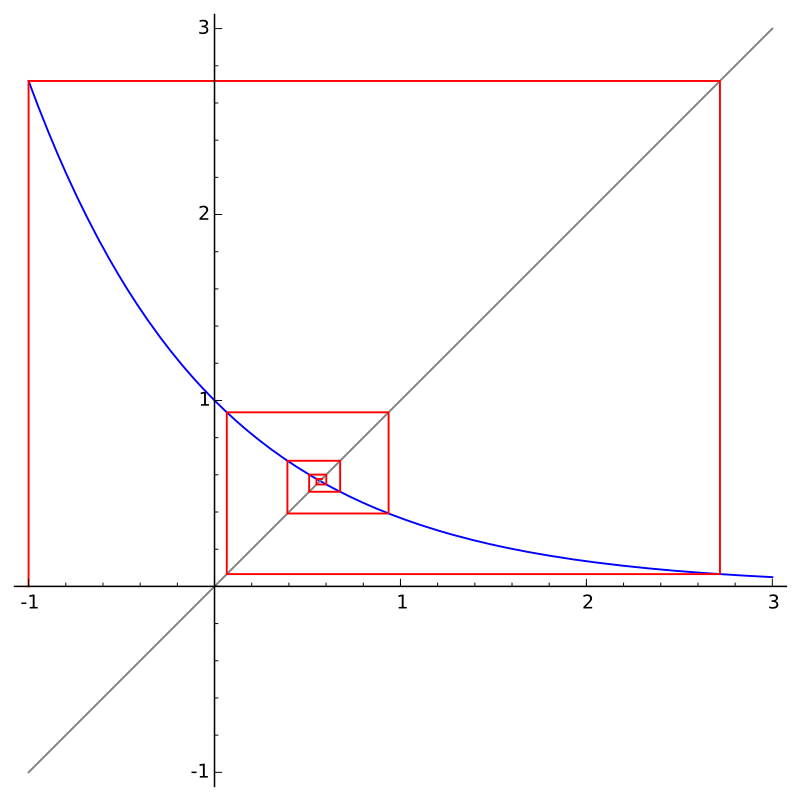
\includegraphics[scale=0.55]{figures/suites-visual1}
\end{center}
\end{frame}

\begin{frame}[fragile]

%On définit la fonction $f(x)=\exp(-x)$ par la commande 
\codeinline{f(x) = exp(-x)}

\pause
%\insertcode{formel/Algos/suites-visual-tex1.sage}{suites-visual.sage (1)}
\begin{algo}[suites-visual.sage (1)]
\begin{lstlisting}
def liste_suite(f,terme_init,n):
    maliste = []
    x = terme_init
    for k in range(n):
        maliste.append(x)
        x = f(x)
    return maliste
\end{lstlisting}
\end{algo}
\pause

\codeinline{liste_suite(f,-1,4)}
\pause
\qquad 
\codeinline{[-1, e, e^(-e), e^(-e^(-e))]}
\end{frame}



\begin{frame}[fragile]

%\insertcode{formel/Algos/suites-visual-tex2.sage}{suites-visual.sage (2)}
\begin{algo}[suites-visual.sage (2)]
\begin{lstlisting}
def liste_points(f,terme_init,n):
    u = liste_suite(f,terme_init,n)
    mespoints = [ (u[0],0) ]
    for k in range(n-1):
        mespoints.append( (u[k],u[k+1]) )
        mespoints.append( (u[k+1],u[k+1]) )
    return mespoints
\end{lstlisting}
\end{algo}

\pause
\codeinline{liste_points(f,-1,3)}
%calcule, pour $a=-1$, le point initial $(-1,0)$ et les $3$ premiers 
%points de la visualisation de la suite $(u_n)$ ;
%on obtient la liste :
affiche :
\centerline{\codeinline{[(-1, 0), (-1, e), (e, e), (e, e^(-e)), (e^(-e), e^(-e))]}}
\end{frame}


\begin{frame}[fragile]

%\insertcode{formel/Algos/suites-visual-tex3.sage}{suites-visual.sage (3)}
\begin{algo}[suites-visual.sage (3)]
\begin{lstlisting}
def dessine_suite(f,terme_init,n):
    mespoints = liste_points(f,terme_init,n)
    G = plot(f,(x,-1,3))      # La fonction
    G = G + plot(x,(x,-1,3))  # La droite (y=x)
    G = G + line(mespoints)   # La suite
    G.show()
\end{lstlisting}
\end{algo}

\pause
%Par exemple la figure illustrant ce tp est construite par la commande

%\begin{tabular}{p{0.20\textwidth}c}
\hfill\hfill\codeinline{dessine_suite(f,-1,10)}

%&
\vbox{\vspace*{-3ex}
\hspace*{2em}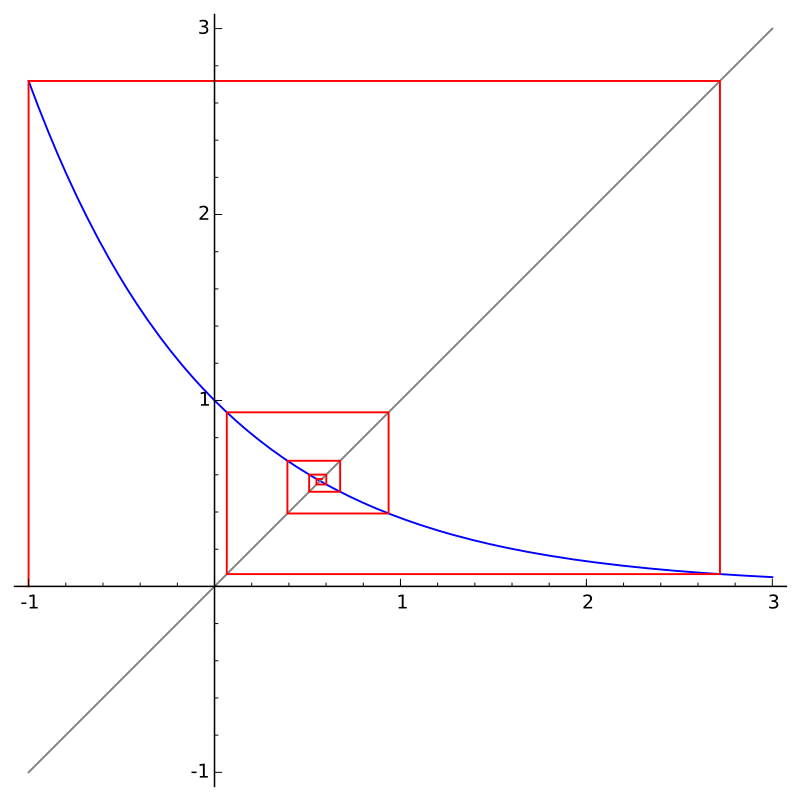
\includegraphics[scale=0.3]{figures/suites-visual1}
}
%\end{tabular}


\end{frame}


%%%%%%%%%%%%%%%%%%%%%%%%%%%%%%%%%%%%%%%%%%%%%%%%%%%%%%%%%%%%%%%%
\section{Listes}

\begin{frame}

\evidence{Listes}

\pause
\begin{itemize}
  
  \item Une liste est présentée entre crochets :
  \codeinline{mesprems = [2,3,5,7,11,13]} \pause
  
  \codeinline{mesprems[i]} ;
  \codeinline{mesprems[0]} vaut $2$,  \codeinline{mesprems[1]} vaut $3$\ldots
  \pause

  \item Parcours d'une liste : \codeinline{for p in mesprems:}
  
  $p$ vaut alors successivement $2$, $3$, $5$, $7$\ldots
  \pause
  \item Création de listes :  partir de la liste vide \codeinline{[]}, \pause
  ajouter un à un des éléments avec \codeinline{append} \pause
  
  \codeinline{mespoints=[]}
  
  \codeinline{mespoints.append((2,3))}
  
  \codeinline{mespoints.append((7,-1))}
  
  \codeinline{mespoints} contient  \codeinline{[ (2,3), (7,-1) ]}

\end{itemize}

\end{frame}


\begin{frame}
\begin{tp}\vspace*{-0.5ex}
Pour $n$ un entier fixé. Composer les listes suivantes :\vspace*{-0.5ex}
\begin{enumerate}
  \item la liste des entiers de $0$ à $n-1$,
  
  \item la liste des entiers premiers strictement inférieurs à $n$,
  
  \item la liste des $2p+1$, pour les premiers $p$ strictement inférieurs à $n$,
  
  \item les $10$ premiers éléments de la liste précédente,
  
  \item la liste de $p_i+i$, où $(p_i)_{i\ge0}$ sont les nombres premiers 
  strictement inférieurs à $n$ ($p_0=2$, $p_1=3$,...),
  
  \item la liste de $1$ et $0$ selon que le rang $0\le k <n$ soit premier ou pas.
\end{enumerate}
\end{tp}
\pause\vspace*{-1ex}
\begin{enumerate}
  \item \codeinline{entiers = range(n)} \pause
  \item \codeinline{premiers = [k for k in range(n) if is_prime(k)]} \pause
  \item \codeinline{doubles = [2*p+1 for p in premiers]} \pause
  \item \codeinline{debut = doubles[0:10]} \pause
  \item \codeinline{prrg= [premiers[i]+i 
		    for i in range(len(premiers))]} \pause
  \item \codeinline{binaire = [zeroun(k) for k in range(n)]} 
  où \codeinline{zeroun(k)} est une fonction qui renvoie $1$ ou $0$ selon que $k$ est premier ou pas 
\end{enumerate}


\end{frame}




%%%%%%%%%%%%%%%%%%%%%%%%%%%%%%%%%%%%%%%%%%%%%%%%%%%%%%%%%%%%%%%%
\section{Suites et chaos}

\begin{frame}
\begin{tp}
On considère la fonction $f$ définie sur $x \in [0,1]$ par 
$$f(x)=rx(1-x) \qquad \text{ où } \quad 0 \le  r \le 4.$$

\pause

Pour $r$ fixé et $u_0 \in [0,1]$ fixé, on définit une suite $(u_n)$ par
$$u_{n+1} = f(u_n).$$

\pause
\begin{enumerate}
  \item Pour différentes valeurs de $r$ et $u_0$ fixées, tracer sur un même graphique
  le graphe de $f$, la droite d'équation $(y=x)$ et la suite $(u_n)$. Essayez de conjecturer 
  le comportement de la suite pour $0<r\le3$, $3< r \le 1+\sqrt{6}$,
  $1+\sqrt{6}< r < 4$ et $r=4$. 
  \end{enumerate}
\end{tp}
\end{frame}


\begin{frame}

$u_0=0,123$ et \only<1>{$r=2,2$}\only<2>{$r=3,2$}\only<3>{$r=3,57$}\only<4>{$r=4$}
  \begin{center}
  \only<1>{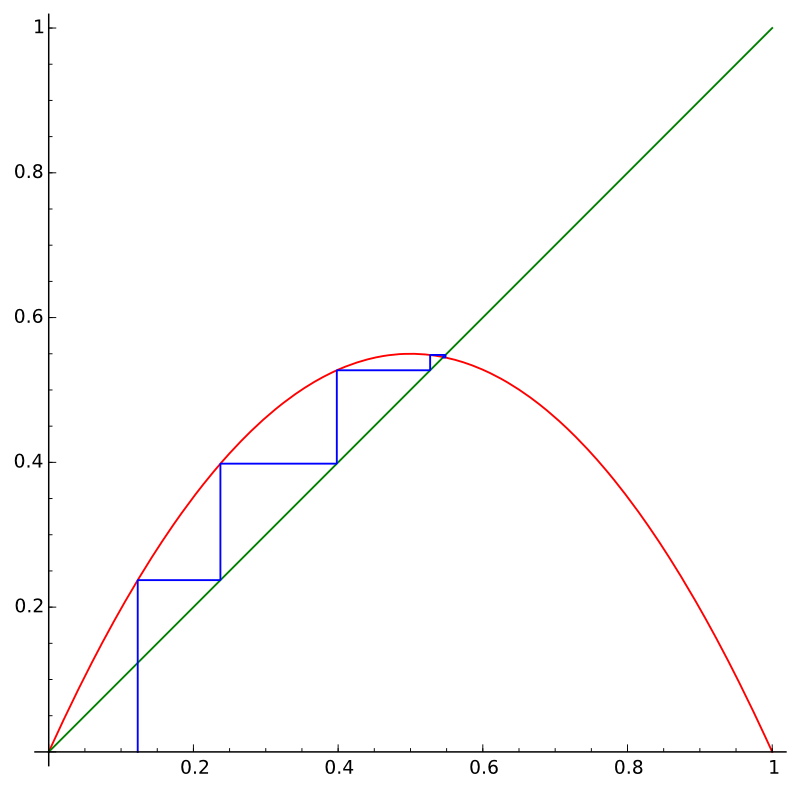
\includegraphics[scale=0.5]{figures/chaos1}}
  \only<2>{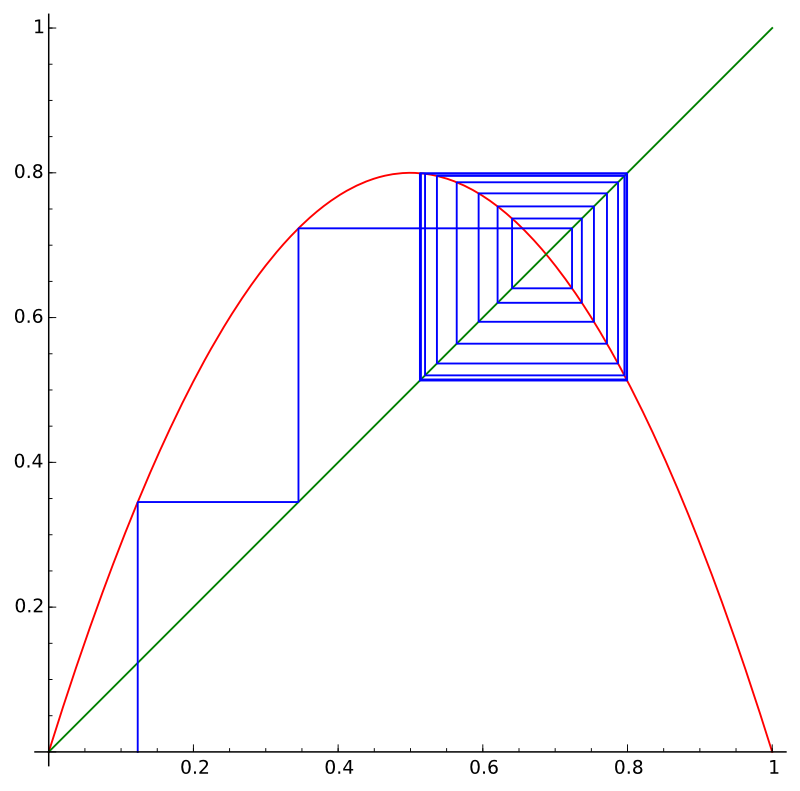
\includegraphics[scale=0.5]{figures/chaos2}}
  \only<3>{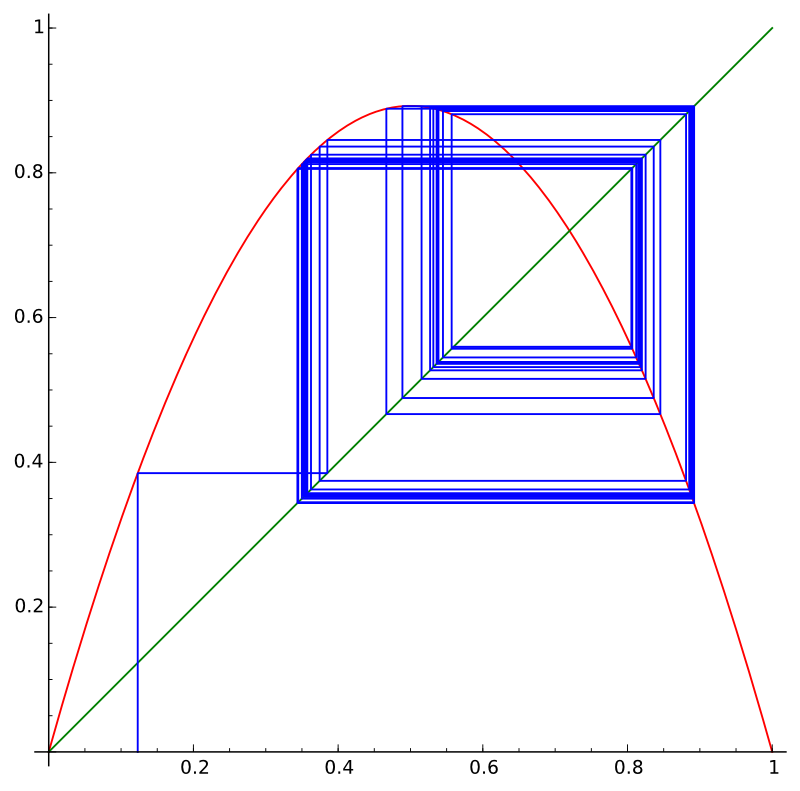
\includegraphics[scale=0.5]{figures/chaos3}}
  \only<4>{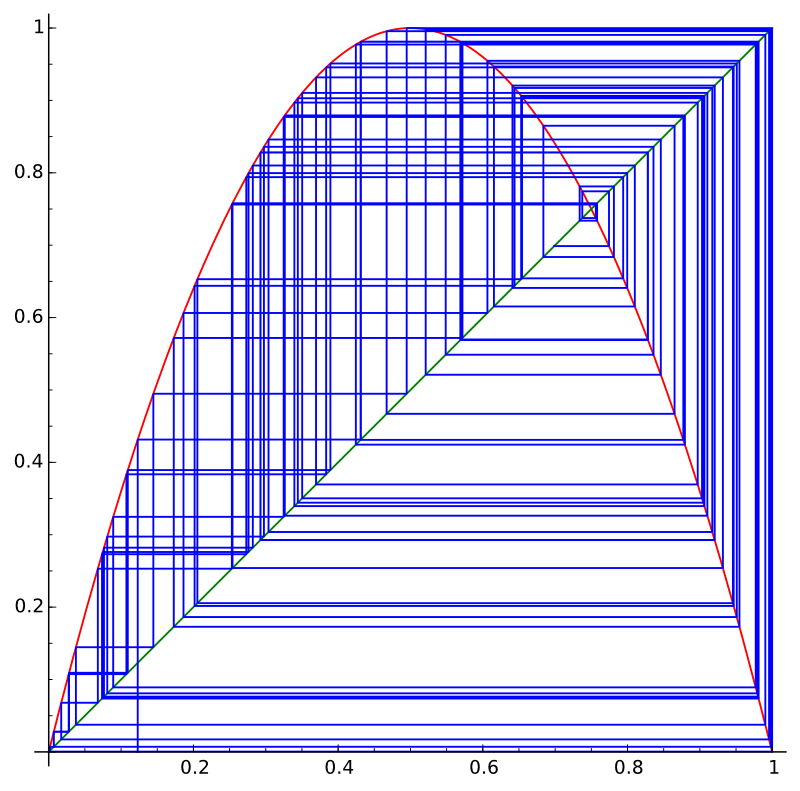
\includegraphics[scale=0.5]{figures/chaos4}} 
  \end{center}
 
\end{frame}
                                                                  



\begin{frame}
\begin{tp}
On considère la fonction $f$ définie sur $x \in [0,1]$ par 
$$f(x)=rx(1-x) \qquad \text{ où } \quad 0 \le  r \le 4.$$

Pour $r$ fixé et $u_0 \in [0,1]$ fixé, on définit une suite $(u_n)$ par
$$u_{n+1} = f(u_n).$$

\pause
\begin{enumerate}
\setcounter{enumi}{1}
 \item Pour $u_0$ fixé et $M<N$ grands (par exemple $M=100$, $N=200$) tracer le \defi{diagramme
  de bifurcation} de $f$, c'est-à-dire l'ensemble des points
  $$(u_i,r) \qquad \text{ pour } \quad M \le i \le N \text{ et } 0 \le r \le 4$$
  \end{enumerate}
\end{tp}
\end{frame}


% \begin{frame}[fragile]
%  %Voici le code et le résultat.
%   
%  % \insertcode{formel/Algos/suites-chaos-tex1.sage}{suites-chaos.sage (1)}
% 
% \begin{algo}[suites-chaos.sage (1)]
% \begin{lstlisting}
% def bifurcation(F,terme_init):
%     Nmin = 100            # On oublie Nmin premiers termes
%     Nmax = 200            # On conserve les termes entre Nmin et Nmax 
%     epsilon = 0.005       # On fait varier r de epsilon à chaque pas
%     r = 2.5               # r initial
%     mespoints = []
%     while r <= 4.0:
%         u = liste_suite(F(r=r),terme_init,Nmax)  # On calcule la suite     
%         for k in range(Nmin,Nmax): 
%             mespoints = mespoints + [(u[k],r)]
%         G = points(mespoints)            
%         r = r + epsilon
%     G.show()
% \end{lstlisting}
% \end{algo}
% 
% 
% \end{frame}

\begin{frame}
 \begin{center}
  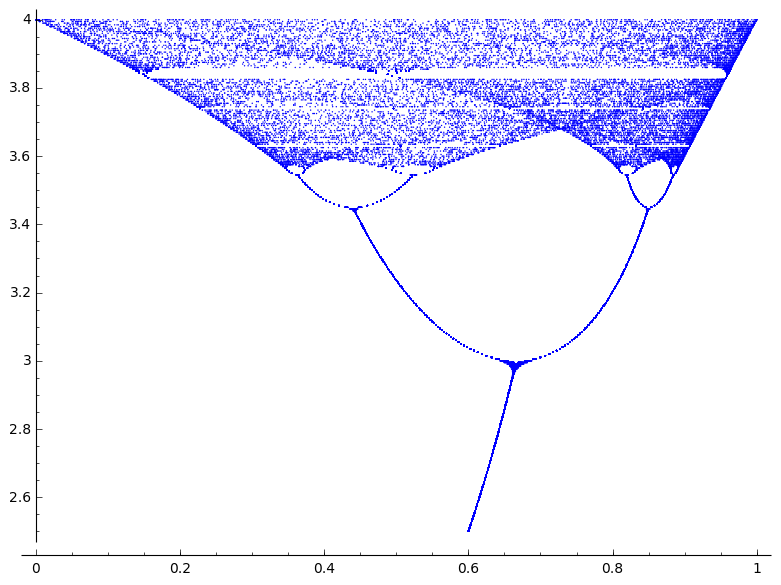
\includegraphics[scale=0.5]{figures/chaos5}  
  \end{center} 

\end{frame}


\begin{frame}
\begin{tp}
On considère la fonction $f$ définie sur $x \in [0,1]$ par 
$$f(x)=rx(1-x) \qquad \text{ où } \quad 0 \le  r \le 4.$$

Pour $r$ fixé et $u_0 \in [0,1]$ fixé, on définit une suite $(u_n)$ par
$$u_{n+1} = f(u_n).$$

\begin{enumerate}
\setcounter{enumi}{2} 
\item \begin{enumerate}
    \item Montrer que les points fixes de $f$ sont $0$ et $\frac{r-1}{r}$.
    \item Montrer que le point fixe $0$ est répulsif (c'est-à-dire $|f'(0)|>1$) dès que $r>1$.
    \item Montrer que le point fixe $\frac{r-1}{r}$ est attractif (c'est-à-dire $|f'(\frac{r-1}{r})|<1$)
    si et seulement si $1< r < 3$. 
  \end{enumerate}  

  \end{enumerate}
\end{tp}
\end{frame}


\begin{frame}[fragile]
%Voici le code pour les trois questions.
    
 % \insertcode{formel/Algos/suites-chaos-tex2.sage}{suites-chaos.sage (2)}
\begin{algo}[suites-chaos.sage (2)]
\begin{lstlisting}
var('x,r')
f(x,r) = r*x*(1-x)
pts_fixes = solve(f==x,x)      # (a) Points fixes
ff = diff(f,x)                 # Dérivée
ff(x=0)                        # (b) f'(0)
solve(abs(ff(x=(r-1)/r))<1,r)  # (c) Point attractif
\end{lstlisting}
\end{algo}
 
% \pause
% \codeinline{[x == (r - 1)/r, x == 0]}
% 
% \pause
% \codeinline{(x, r) |--> -(x - 1)*r - r*x}
% 
% \pause
% \codeinline{r}
% 
% \pause
% \codeinline{[[1 < r, r < 3]]}
\pause
    \begin{itemize}
    \item \codeinline{pts_fixes} renvoie $0$ et $\frac{r-1}{r}$
    \pause
    \item $f'(0)=r$. Si $r>1$ alors $0$ est un point répulsif
    \pause
    \item L'inéquation $|f'(\frac{r-1}{r})|<1$, équivaut à $1<r<3$, 
    le point fixe $\frac{r-1}{r}$ est alors attractif
  \end{itemize} 

\end{frame}

\begin{frame}
\begin{tp}
On considère la fonction $f$ définie sur $x \in [0,1]$ par 
$$f(x)=rx(1-x) \qquad \text{ où } \quad 0 \le  r \le 4.$$

Pour $r$ fixé et $u_0 \in [0,1]$ fixé, on définit une suite $(u_n)$ par
$$u_{n+1} = f(u_n).$$

\begin{enumerate}
\setcounter{enumi}{3} 
\item \textbf{Cas $1 < r \le3$. Pour $0<u_0<1$ la suite $(u_n)$ converge vers $\frac{r-1}{r}$.}
 
  On va prouver ce résultat seulement dans le cas particulier $r=2$ :
  \begin{enumerate}
    \item Montrer que $u_{n+1}-\frac12 = -2\left(u_n-\frac12\right)^2$.
    \item Montrer que si $|u_0-\frac12| < k < \frac12$ alors 
    $|u_n-\frac12| < \frac12 (2k)^{2^n}$.
    \item Conclure.
  \end{enumerate} 

  \end{enumerate}
\end{tp}
\end{frame}



% \begin{frame}
%  On pose d'abord \codeinline{r = 2}, alors le point fixe est $\frac{r-1}{r}= \frac12$.
%   \begin{enumerate}
%     \item Après simplification \codeinline{(r*u*(1-u) - 1/2) + 2*(u-1/2)^2} vaut $0$.
%     Autrement dit $u_{n+1}-\frac12 = -2(u_n-\frac12)^2$, quelque soit $u_n$.
%     \item C'est une simple récurrence :
%     $$\left|u_{n+1}-\frac12\right|  = 2 \left(u_n-\frac12\right)^2 
%     < 2\left(\frac12 (2k)^{2^n}\right)^2 = \frac12 (2k)^{2^{n+1}}.$$
%     \item Ainsi pour $u_0 \neq 0,1$, il existe $k$ tel que $|u_0-\frac12| < k < \frac12$
%     et la suite $(u_n)$ tend (très très) vite vers le point fixe $\frac12$.
%   \end{enumerate} 
% \end{frame}


\begin{frame}

  $r=2$
  \begin{center}
  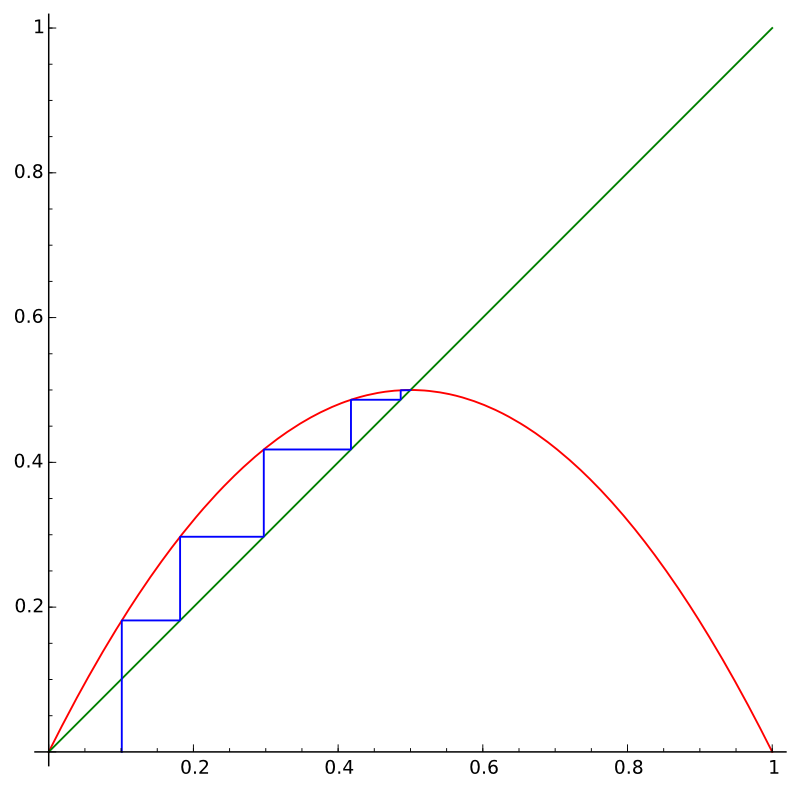
\includegraphics[scale=0.5]{figures/chaos6}  
  \end{center}   

\end{frame}

% \begin{frame}[fragile]
% \begin{tp}
% On considère la fonction $f$ définie sur $x \in [0,1]$ par 
% $$f(x)=rx(1-x) \qquad \text{ où } \quad 0 \le  r \le 4.$$

% Pour $r$ fixé et $u_0 \in [0,1]$ fixé, on définit une suite $(u_n)$ par
% $$u_{n+1} = f(u_n).$$

% \begin{enumerate}
% \setcounter{enumi}{3} 
% \item
	 % \textbf{Cas $3<r<1+\sqrt{6}$. La suite $(u_n)$ possède un cycle attracteur de période $2$.}
   
  % \begin{enumerate}
    % \item Déterminer les points fixes $\ell_1$ et $\ell_2$ de $f\circ f$ qui ne sont pas des points fixes 
    % de $f$.
     
    % \item Montrer que $f(\ell_1) = \ell_2$ et $f(\ell_2)=\ell_1$.
     
    % \item \`A l'aide du graphe de $f\circ f$, vérifier graphiquement sur un exemple, 
    % que les suites $(u_{2n})$ et $(u_{2n+1})$ sont croissantes ou décroissantes à partir d'un certain rang
    % et convergent, l'une vers $\ell_1$, l'autre vers $\ell_2$.
  % \end{enumerate} 

  % \end{enumerate}
% \end{tp}
% \end{frame}



% \begin{frame}

% \end{frame}

\begin{frame}[fragile]
\begin{tp}
On considère la fonction $f$ définie sur $x \in [0,1]$ par 
$$f(x)=rx(1-x) \qquad \text{ où } \quad 0 \le  r \le 4.$$

Pour $r$ fixé et $u_0 \in [0,1]$ fixé, on définit une suite $(u_n)$ par
$$u_{n+1} = f(u_n).$$

\begin{enumerate}
\setcounter{enumi}{4} 
\item
\textbf{Cas $3<r<1+\sqrt{6}$. La suite $(u_n)$ possède un cycle attracteur de période $2$.}
\pause 
  \begin{enumerate}
    \item Déterminer les points fixes $\ell_1$ et $\ell_2$ de $f\circ f$ qui ne sont pas des points fixes 
    de $f$.
 \pause     
    \item Montrer que $f(\ell_1) = \ell_2$ et $f(\ell_2)=\ell_1$.
  \pause      
    \item \`A l'aide du graphe de $f\circ f$, vérifier graphiquement sur un exemple, 
    que les suites $(u_{2n})$ et $(u_{2n+1})$ sont croissantes ou décroissantes à partir d'un certain rang
    et convergent, l'une vers $\ell_1$, l'autre vers $\ell_2$.
  \end{enumerate} 

  \end{enumerate}
\end{tp}
\end{frame}



\begin{frame}[fragile]
% \insertcode{formel/Algos/suites-chaos-tex3.sage}{suites-chaos.sage (3)}
\begin{algo}[suites-chaos.sage (3)]
\begin{lstlisting}
var('x,r')
f(x,r) = r*x*(1-x)             # f
g = f(x=f(x,r))                # g(x) = f(f(x))
pts_doubles = solve(g==x,x)    # (a) Points fixes de g
# Les deux nouveaux points fixes de g :
ell1 = pts_doubles[0].rhs()
ell2 = pts_doubles[1].rhs()
eq = f(x=ell1)-ell2            # (b) f(ell1)=ell2 ?
eq.full_simplify()             # Oui !
\end{lstlisting}
\end{algo}

\pause
 \begin{itemize}
    \item Deux points fixes de $g = f\circ f$ qui ne sont pas des points fixes de $f$   
    $$\ell_1 = \frac12\frac{r + 1 - \sqrt{r^2 - 2r - 3}}{r} \qquad 
      \ell_2 = \frac12\frac{r + 1 + \sqrt{r^2 - 2r - 3}}{r}$$
     
  \vspace*{-2ex}   
  
\pause      
    \item $f(\ell_1) = \ell_2$ (et d'où $f(\ell_2)=\ell_1$)
 \end{itemize}
\end{frame}

\begin{frame}

Pour $r=1+\sqrt{5}$ et $u_0=\frac23$
 
    \`A gauche : suite $(u_{2n})$, vue comme suite récurrente de $g$, 
    est décroissante vers $\ell_1$
    
    \`A droite : suite $(u_{2n+1})$, vue comme suite récurrente de $g$,
    est croissante vers $\ell_2$


  \begin{center}
  \hspace*{-3em}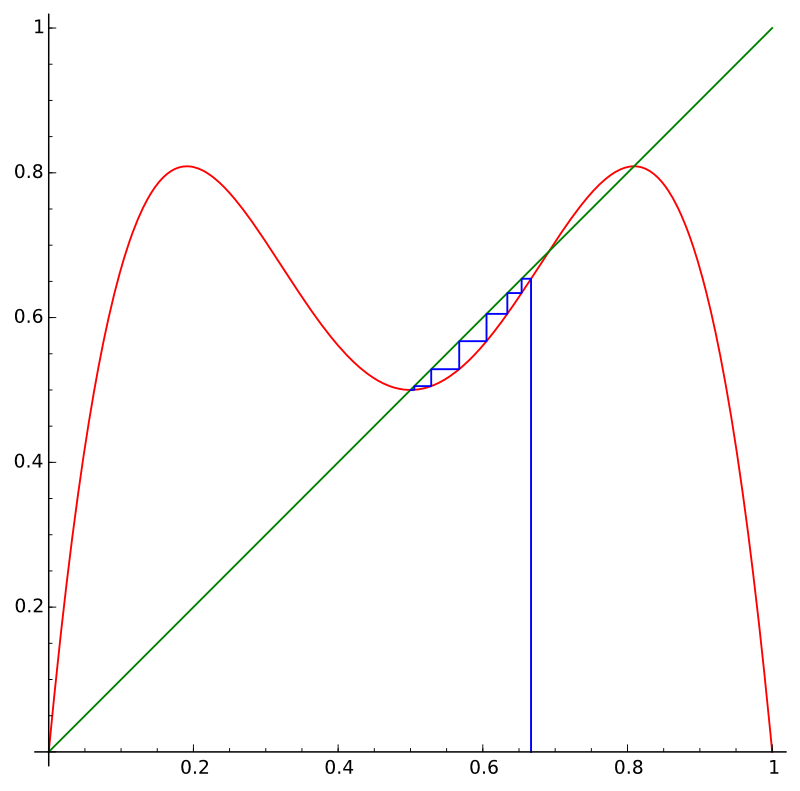
\includegraphics[scale=0.4]{figures/chaos7}\quad 
  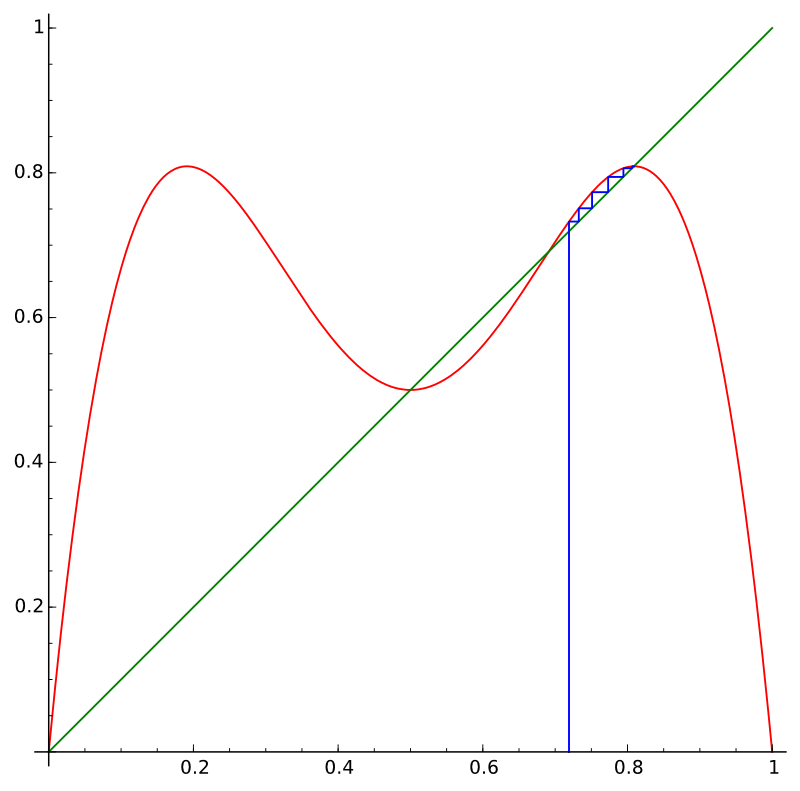
\includegraphics[scale=0.4]{figures/chaos8}
  \end{center}
\end{frame}


\begin{frame}
  La suite $(u_n)$, comme suite récurrente de fonction $f$, possède 
  le cycle $(\ell_1,\ell_2)$ comme cycle attracteur
  \begin{center}
  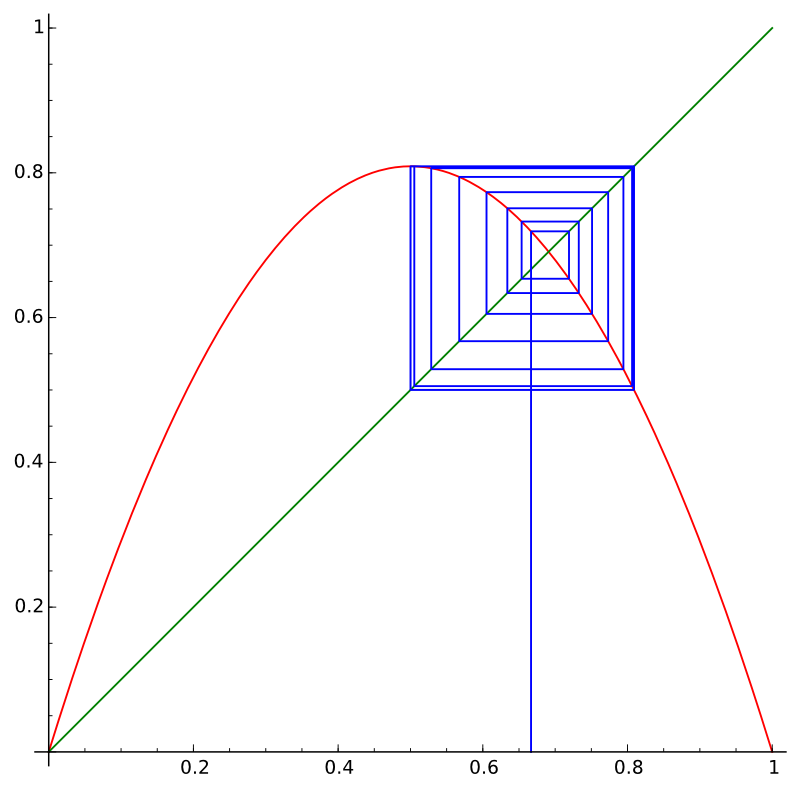
\includegraphics[scale=0.5]{figures/chaos9}
  \end{center} 

\end{frame}


\begin{frame}
\begin{tp}
On considère la fonction $f$ définie sur $x \in [0,1]$ par 
$$f(x)=rx(1-x) \qquad \text{ où } \quad 0 \le  r \le 4.$$

Pour $r$ fixé et $u_0 \in [0,1]$ fixé, on définit une suite $(u_n)$ par
$$u_{n+1} = f(u_n).$$

\begin{enumerate}
\setcounter{enumi}{5} 
 \item \textbf{Cas $1+\sqrt{6}<r<3, 5699456\ldots$ La suite $(u_n)$ possède 
  un cycle attracteur de période $4,8,16...$}
  
  Trouver de tels exemples.    

  \item \textbf{\`A partir de $r > 3, 5699456\ldots$ la suite $(u_n)$ devient chaotique.}



  \end{enumerate}
\end{tp}
\end{frame}



\begin{frame}
\begin{enumerate}
  \setcounter{enumi}{5}
  \item Exemple de cycle de longueur $8$ (pour $r=3,56$, $u_0=0,35$)
 \end{enumerate} 
   \begin{center}
   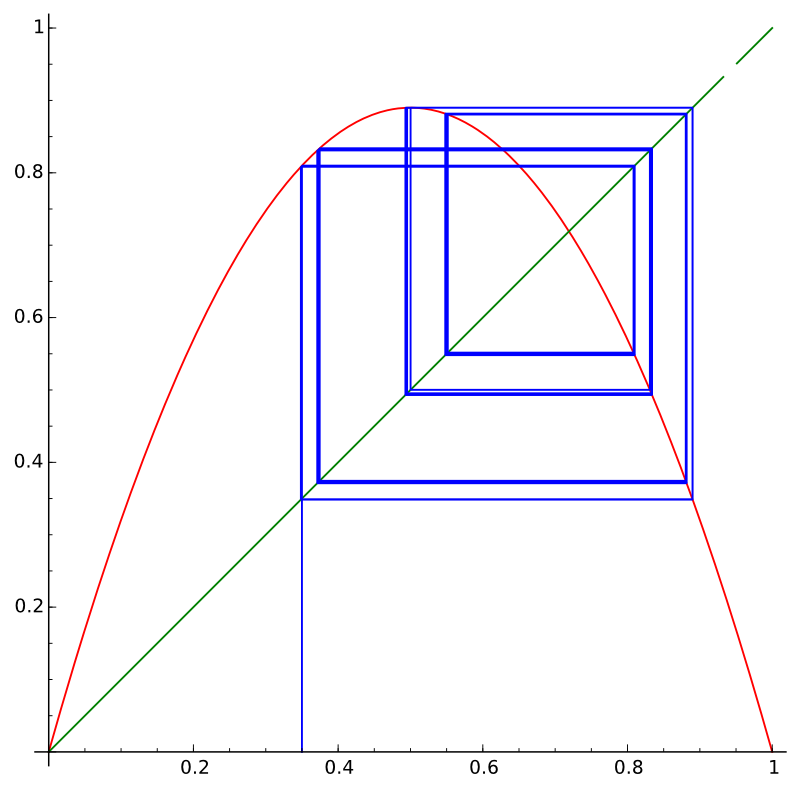
\includegraphics[scale=0.5]{figures/chaos10}  
   \end{center}

 \end{frame}



\begin{frame} 
\begin{enumerate}
\setcounter{enumi}{6}
  \item $r=4$ : le chaos
  \end{enumerate} 
  \begin{center}
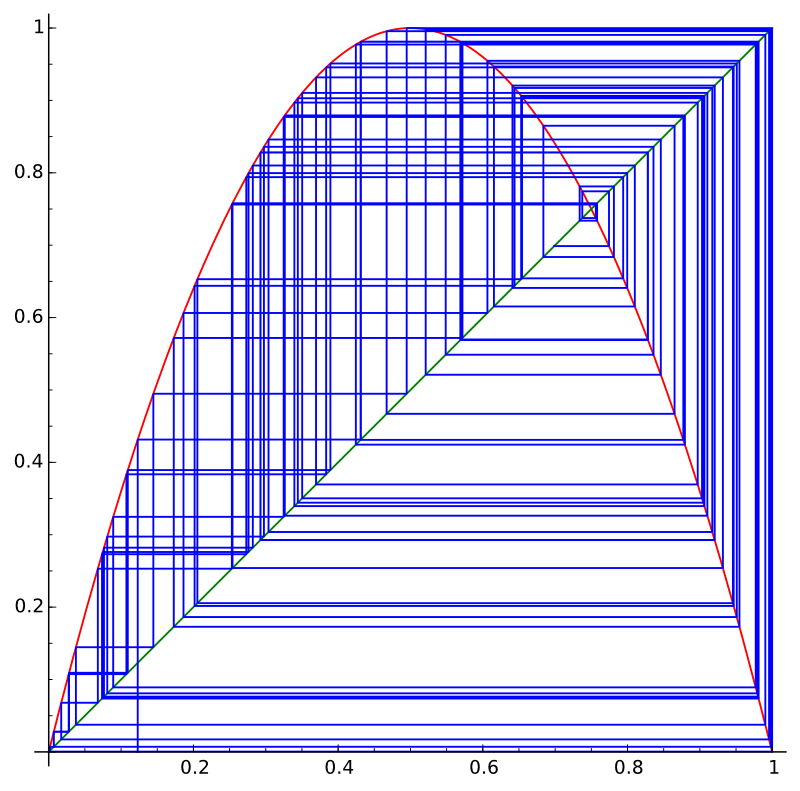
\includegraphics[scale=0.5]{figures/chaos4}
  \end{center}



\end{frame}


\end{document}
